\documentclass[11pt]{book}

\usepackage[ruled,vlined]{algorithm2e}
\usepackage[utf8]{inputenc}

\usepackage{graphicx} 
\usepackage{amsfonts}
\usepackage{amssymb}
\usepackage{amsmath}

\usepackage[pdftex]{color, hyperref}
\hypersetup{colorlinks,%
	citecolor=black,%
	filecolor=black,%
	linkcolor=black,%
	urlcolor=black,%
}
\pdfpagewidth=\paperwidth
\pdfpageheight=\paperheight

% package `subfigure` and `subfig` are deprecated and should not be used
% unless withing the IEEETran or ACM SIG templates
\usepackage{subcaption}

% To handle the acronyms nicely
\usepackage[nonumberlist, toc, acronym]{glossaries}
\newacronym{csma}{CSMA}{Carrier Sense Multiple Access}
\newacronym{fdd}{FDD}{Frequency Division Duplexing}
\newacronym{tdd}{TDD}{Time Division Duplexing}
\newacronym{fdma}{FDMA}{Frequency Division Multiple Access}
\newacronym{tdma}{TDMA}{Time Division Multiple Access}
\newacronym{cdma}{CDMA}{Code Division Multiple Access}
\newacronym{wcdma}{WCDMA}{Wide-band Code Division Multiple Access}
\newacronym{ss}{SS}{Spread Spectrum}
\newacronym{sdma}{SDMA}{Space Division Multiple Access}
\newacronym{ofdm}{OFDM}{Orthogonal Frequency Division Multiplexing}
\newacronym{ofdma}{OFDMA}{Orthogonal Frequency Division Multiple Access}
\newacronym{ufr}{UFR}{Universal Frequency Reuse}
\newacronym{4g}{4G}{4$^{th}$ Generation of Mobile Communications}
\newacronym{3g}{3G}{3$^{rd}$ Generation of Mobile Communications}
\newacronym{3gpp}{3GPP}{3$^{rd}$ Generation Partnership Project}
\newacronym{hspa+}{HSPA+}{High-Speed Packet Access Plus}
\newacronym{lte}{LTE}{Long Term Evolution}
\newacronym{ltea}{LTE-A}{Long Term Evolution Advanced}
\newacronym{mimo}{MIMO}{Multiple Input Multiple Output}
\newacronym{itu}{ITU}{International Telecommunication Union}
\newacronym{itur}{ITU-R}{International Telecommunication Union Radiocommunication Sector}
\newacronym{imta}{IMT-Advanced}{International Mobile Telecommunications-Advanced}
\newacronym{ca}{CA}{Carrier Aggregation}
\newacronym{rn}{RN}{Relay Node}
\newacronym{comp}{CoMP}{Coordinated Multi Point}

\makeglossaries

% To handle the references
\usepackage{natbib}

%%%%%%%%%%%%%%%%%%%%%%%%%%%%%%%%%%%%%%%%%%%%%%%%%%%%%%%%%%%%%%%%%%%%%%%%%%%%%%%%
\newcommand{\refs}[1]{Section~\ref{#1}}
\newcommand{\refss}[1]{Subsection~\ref{#1}}
\newcommand{\reff}[1]{Figure~\ref{#1}}

%%%%%%%%%%%%%%%%%%%%%%%%%%%%%%%%%%%%%%%%%%%%%%%%%%%%%%%%%%%%%%%%%%%%%%%%%%%%%%%%
% Margins
%\setlength{\textheight}{22cm}
%\setlength{\headsep}{1cm}
%\setlength{\topmargin}{-0.5cm}
%\setlength{\textwidth}{14cm}
\setlength{\oddsidemargin}{2cm}
\setlength{\evensidemargin}{2cm}

% Include up to subsections in the TOC
\setcounter{tocdepth}{3}

% So that the empty pages have no page number
\makeatletter
  \def\cleardoublepage{\clearpage\if@twoside \ifodd\c@page\else
  \vspace*{\fill}
    \thispagestyle{empty}
    \newpage
    \if@twocolumn\hbox{}\newpage\fi\fi\fi}
\makeatother

%%%%%%%%%%%%%%%%%%%%%%%%%%%%%%%%%%%%%%%%%%%%%%%%%%%%%%%%%%%%%%%%%%%%%%%%%%%%%%%%
% PREFACE
%%%%%%%%%%%%%%%%%%%%%%%%%%%%%%%%%%%%%%%%%%%%%%%%%%%%%%%%%%%%%%%%%%%%%%%%%%%%%%%%
\begin{document}

% \frontmatter
% % First part uses roman numbering
\pagenumbering{gobble}
% \cleardoublepage
% {\Large

% \begin{figure}[t]
% 	\centering
% 	\centerline{  
% 	
\includegraphics[width=3.5cm]{./ch0/logo.uc3mGrande.eps} 
% 	} 
% \end{figure}


\centerline{UNIVERSIDAD CARLOS III DE MADRID}

\centerline{Departamento de Teoría de la Señal y Comunicaciones}


\vspace*{2.5cm}
\centerline{DOCTORAL THESIS}

\vspace*{1cm}
\begin{center}
{\bf
	BLOCK DIAGONALIZATION TECHNIQUES FOR CELLULAR NETWORKS: CLUSTERING AND SCHEDULING
}
\end{center}

\vspace*{3cm}
Author: JUAN JOSÉ GARCÍA FERNÁNDEZ

Advisor: ANA GARCÍA ARMADA

Date: TBD (Hopefully not far from now)

} % Large

% \newpage
% 
% \cleardoublepage
% \begin{tabular}{l l}
{\bf Tesis Doctoral:} 
& BLOCK DIAGONALIZATION TECHNIQUES\\
& FOR CELLULAR NETWORKS:\\
& CLUSTERING AND SCHEDULING\\
\\
{\bf Autor:} 
& Juan José García Fernández\\
\\
{\bf Director:} 
& Dra. Ana García Armada
\\
\end{tabular}


\vspace*{2cm}

{\large El tribunal nombrado para juzgar la tesis doctoral arriba citada, compuesto por los doctores}


\vspace*{1cm}

Presidente:

\vspace*{2cm}

Vocal:


\vspace*{2cm}

Secretario:

\vspace{2cm}
{\large acuerda otorgarle la calificación de}

\vspace{2cm}
{\large Leganés, a}

% \newpage
% 
% \cleardoublepage
% \chapter*{Agradecimientos}
\markright{Agradecimientos}

Mi primer y más importante agradecimiento va dirigido a mis padres. Por
respetar mis erráticos pasos por este mundo, incluso cuando no los compartían.
Siempre han estado ahí, como un contrafuerte sobre el que apoyar la carga de las
preocupaciones, cuando ha sido necesario. Mi hermana, en la distancia, también
ha sido participe de que sea como soy y quien soy ahora mismo. Ella pasó por lo
mismo pero, como siempre le ha ocurrido, sin un hermano mayor a quien recurrir,
haciéndolo más difícil. Gracias a ellos, llegar a este punto no ha sido tan
difícil como me gusta decir.

Y es que me he quejado mucho durante este tiempo, pero como dicen mis amigos los
pollos, ``he vivido como he querido''. En los últimos tiempos me he distanciado
de ellos, pero sé que siempre están ahí si realmente necesito algo de ellos, de
forma desinteresada, por ello quiero darles las gracias.

No me puedo olvidar, aunque lo había hecho, de Julio, José y Rober (y Bea cuando
se digna), que con esporádicos frikimiércoles han mantenido viva la chispa de la
curiosidad por cosas diferentes, cada uno hablándonos de nuestras cosas.

Por supuesto, con quien más tiempo he pasado, al final, ha sido con mis
compañeros de laboratorio, Máximo, Özge, Javier, Alex, Alex (el orden lo elegís
vosotros), Borja, Cecilia. En el fondo son la principal razón por la que merecía
la pena ir cada día a la universidad. Antes que todos ellos, Omar estuvo ahí, y
juntos compartimos penurias y lamentos, de los que espero que nos vayamos
librando poco a poco. A tita Sara tengo que agradecerle su optimismo resignado,
siempre enfrentándose a la dura realidad con una visión positiva. Lo mejor es
que ahora volveré a compartir tiempo con ella$\ldots$ un aliciente más para
afrontar el siguiente paso. Con un optimismo ligeramente diferente, Jair siempre
ha servido de motivación para seguir adelante. Su visión del mundo de la
universidad realmente llegaba a calar, y me hizo comprender, en ocasiones, que
no todo era tan negro como lo veía.

A mi tutora, Ana, he de agradecerle su optimismo infatigable y su capacidad para
ver lo bueno en todo, y por su paciencia aguantándome.

During the time I spent in the USA, I met very special people. First I want to
thank Nima and Tommi, because they were (and still are, from afar) true friends,
and made the life much easier in there. It is always a relief finding people who
are so similar to me, so far from home. Meo appeared at some point, too, with
her capacity to joke about almost anything, but still be serious when needed.
And she appeared through the most special person I met there, Samar. I spent
with her the most precious time I have spent with anyone in the recent years.
Despite the distance, she is still so important for me. I want to thank her
because she was the main reason to continue with the PhD, her selfless support
kept me focused and gave me strength to not give up. I want to truly thank her
for having so much faith in me.

Aparte de los compañeros de laboratorio, las actividades deportivas han sido
otro de los pilares que me han mantenido en pie. La natación y el aikido me han
dado la vida, a través de la salud. A mis monitores de natación (Jesús y Gema),
y a mi sensei (Julio) he de agradecerles sus esfuerzos. Y a mis compañeros de
aikido Borja, Gerardo, Javier y Rodolfo, agradecerles la posibilidad de entrenar
y crecer juntos.

Finalmente quiero agradecer el apoyo recibido de múltiples otros amigos y
amigas, que con el tiempo que me han dedicado han conseguido que pudiera
respirar a través de las brumas del desánimo. Unos más recientes, otros más
antiguos, su aportación ha sido igualmente importante: Carlos, Diego, Esther,
Isaac, Lydia, Marcos.

% \newpage
% 
% \cleardoublepage
% \pagenumbering{Roman}
% \chapter*{Abstract}

The need for higher data rates and higher efficiency in cellular networks
motivates the use of \gls{ufr}. Coordination among \glspl{bs} is required then
to alleviate the performance penalty due to the interference. Global
coordination is too complex and has inherent limitations that prevents it from
being used in real world scenarios. Clusters of a reduced number of \glspl{bs}
can be considered in order to ease off the requirements of coordination. As a
result, \gls{oci} appears, affecting negatively the communications.

This work focuses on \gls{bd}, a linear precoding technique that combines a
good theoretical performance with a relatively low complexity. However, the
unwanted interference seriously impacts the results obtained using \gls{bd}.

This thesis studies the downlink of a clustered cellular network, where \gls{bd}
is used to coordinate the \gls{bs} within each cluster. The mean achievable rate
is analyzed as a function of several scenario parameters. Of particular interest
is the dependence on the cluster size, which yields that there is an optimum
cluster size, beyond which no significant gain is obtained. Fairness
considerations are analyzed in the presence of \gls{oci}, also studied as a
function of scenario parameters such as the power allocation.

A mixed strategy using \gls{bd} and \gls{su} processing is proposed as a means
to overcome the impairment of the unhandled interference. The transmission
consists of two stages:

\begin{itemize}
    \item Users locally decide which transmission strategy they prefer and send
        this information to the \glspl{bs}.
    \item \glspl{bs} use the decisions of all users to schedule them for
        transmission so that the performance of the network is optimized.
\end{itemize}

The result of the proposed strategy is an improvement in the performance of
\gls{bd} in the presence of \gls{oci}, especially for the users experiencing the
worst conditions. This means that the fairness of the system is also increased,
along with the overall performance of the network.

% \newpage
% 
% \cleardoublepage
% {\Huge {\bf Resumen}}

\lipsum[5]

% \newpage

% Index
\tableofcontents{}

% List of tables and Figures
% \addcontentsline{toc}{chapter}{\protect\numberline{}{Lista de tablas}}
\listoftables{}
\listoffigures{}

% Acronyms
\printglossary[type=\acronymtype]

\mainmatter
%%%%%%%%%%%%%%%%%%%%%%%%%%%%%%%%%%%%%%%%%%%%%%%%%%%%%%%%%%%%%%%%%%%%%%%%%%%%%%%%
% CHAPTERS
%%%%%%%%%%%%%%%%%%%%%%%%%%%%%%%%%%%%%%%%%%%%%%%%%%%%%%%%%%%%%%%%%%%%%%%%%%%%%%%%

% % Back to arabic numbering
% \pagenumbering{arabic}

% Introduction
\chapter{Introduction}\label{ch:intro}

Every new generation of cellular network technologies comes with a new set of
requirements, dictated by the trends in the use of the mobile connectivity. A
common requirement to every single generation is their striving for higher data
rates and greater power efficiency. This motivates research and techology
innovation in order to achieve the goals set for each generation.


The research associated usually requires revisiting old paradigms used in
previous generations, and updating them with novel ideas.


The \emph{release 7} of the \gls{3gpp} \gls{3g} specifications \citep{3Grel7},
also known as \gls{hspa+}, inluded the use of \gls{mimo} as a means to increase
the rates of transmission.


\emph{Release 8}, more well known by its commercial name \gls{lte} \citep{3gpplte},
introduced a new physical layer, based on \gls{ofdm} instead of \gls{wcdma} as in
\gls{3g}. Although the rates attainable with \gls{wcdma} may be comparable to those
obtained with \gls{ofdm}, the latter provides a much easier equalization mechanism
that makes dealing with multipath channels a simpler task. Apart from that \gls{ofdm}
provides a higher flexibility in the resource allocation and user and enables the
use of \gls{ofdma}.

\gls{lte} did not meet the requirements issued by the \gls{itur} \gls{imta} radio
interface \citep{imta} for what is known as \gls{4g} though.

The introduction of \gls{ltea} in \emph{release 10} of the LTE specification
\citep{3gppltea} met the requirements to be considered an \gls{imta} system. The main
novelties included in \gls{ltea} are \gls{ca}, enhanced use of MIMO techniques and support
for \gls{rn}.

\emph{Release 11} \citep{lterel11} included in the specification the support for
\gls{comp} operation. \gls{comp} was included in order to improve the network
performance at cell edges, for it uses several transmitters to provide coordinated
transmission in the downlink, and a number of receivers to provide coordinated
reception in the uplink.

The \gls{comp} operation considered in \citep{lterel11} is just a part of a much
broader field of multi-cell cooperation or coordinated communications where several
cells are assumed to cooperate, in the sense that they take measures in order to
alleviate to a certain degree the level of interference introduced into other parts
of the network, or the use of that interference to their advantage.

\begin{figure}[t]
    \centering
    \begin{subfigure}[b]{0.45\textwidth}
        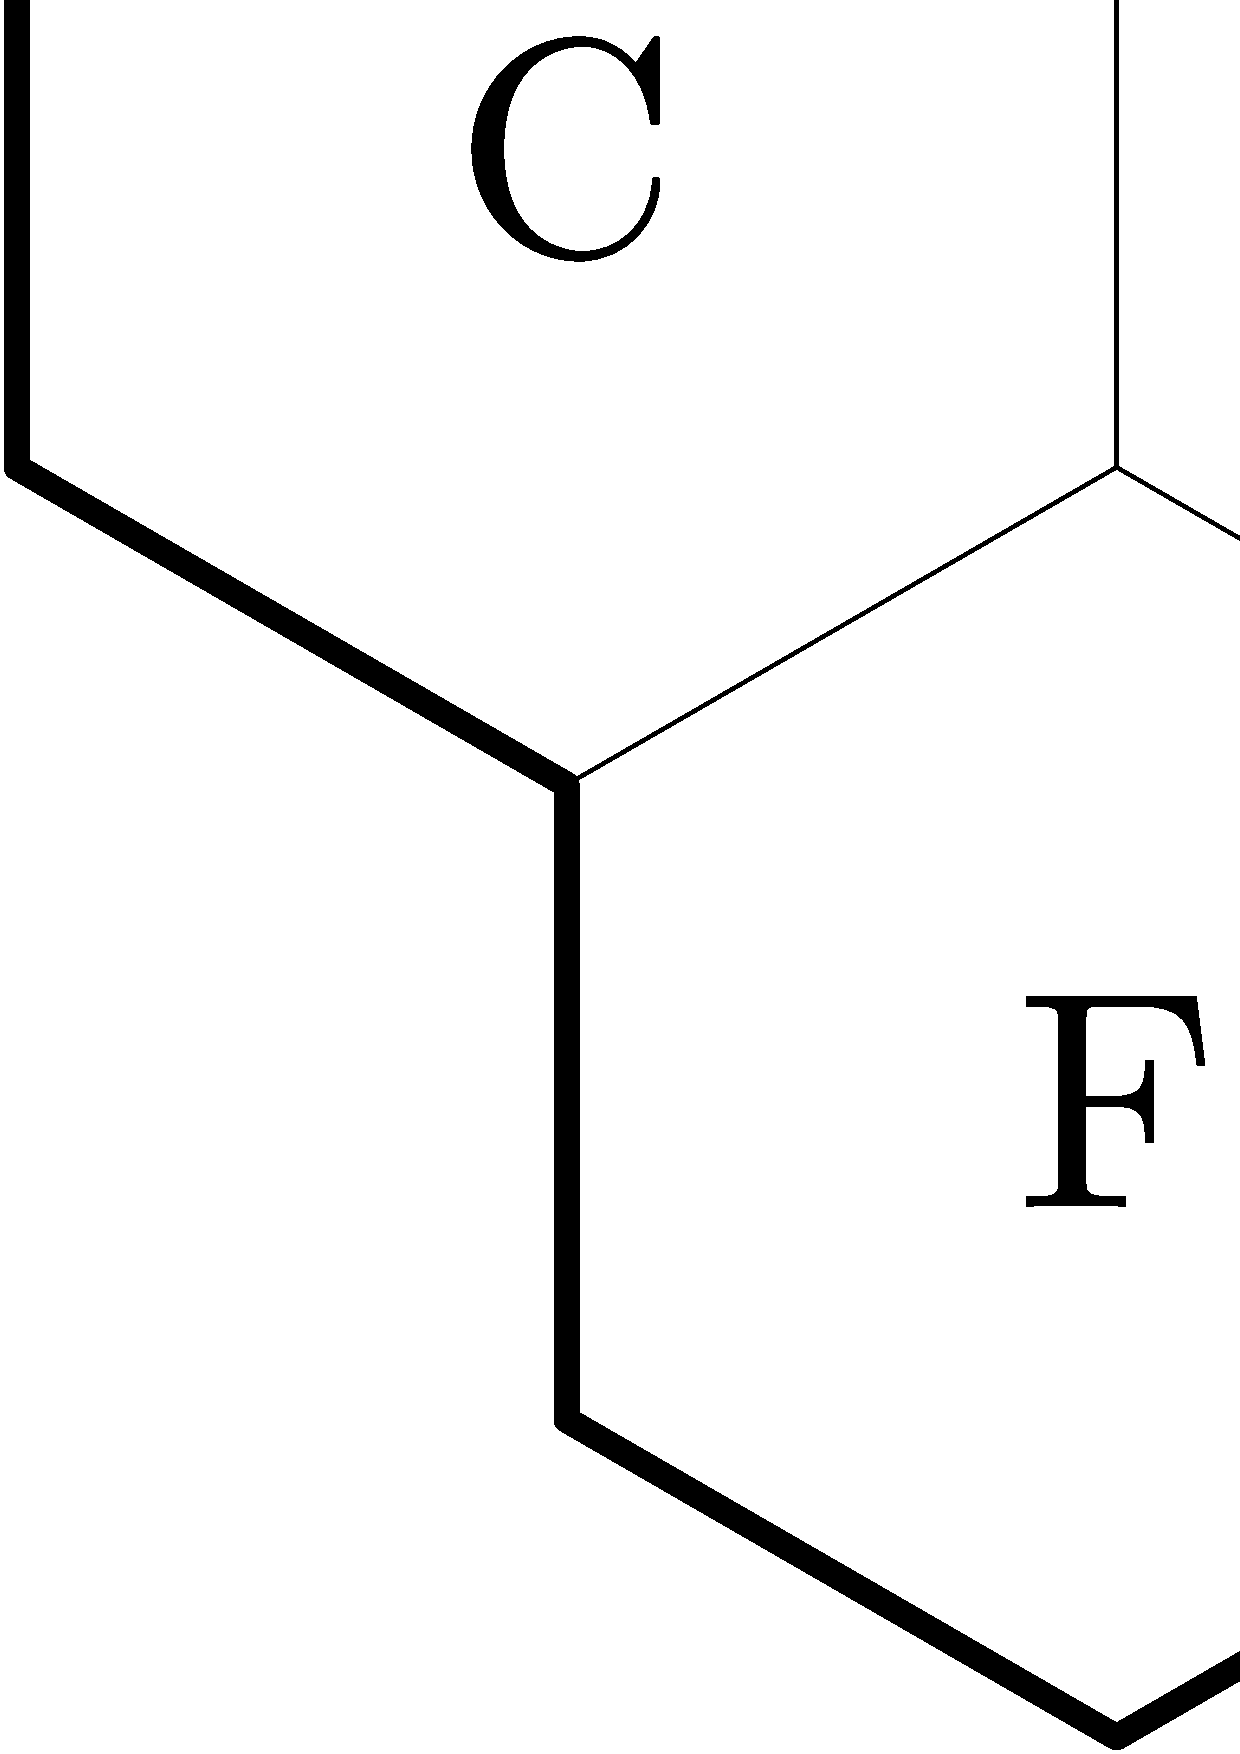
\includegraphics[width=\textwidth]{./ch1/img/frequency_reuse.png}
        \caption{Frequency reuse factor of $1 / 7$.}
        \label{fig:freuse}
    \end{subfigure}
    % Comment out the line break that is introduced with the blank line
    % so that it does not put the images one on top of the other...
    \begin{subfigure}[b]{0.45\textwidth}
        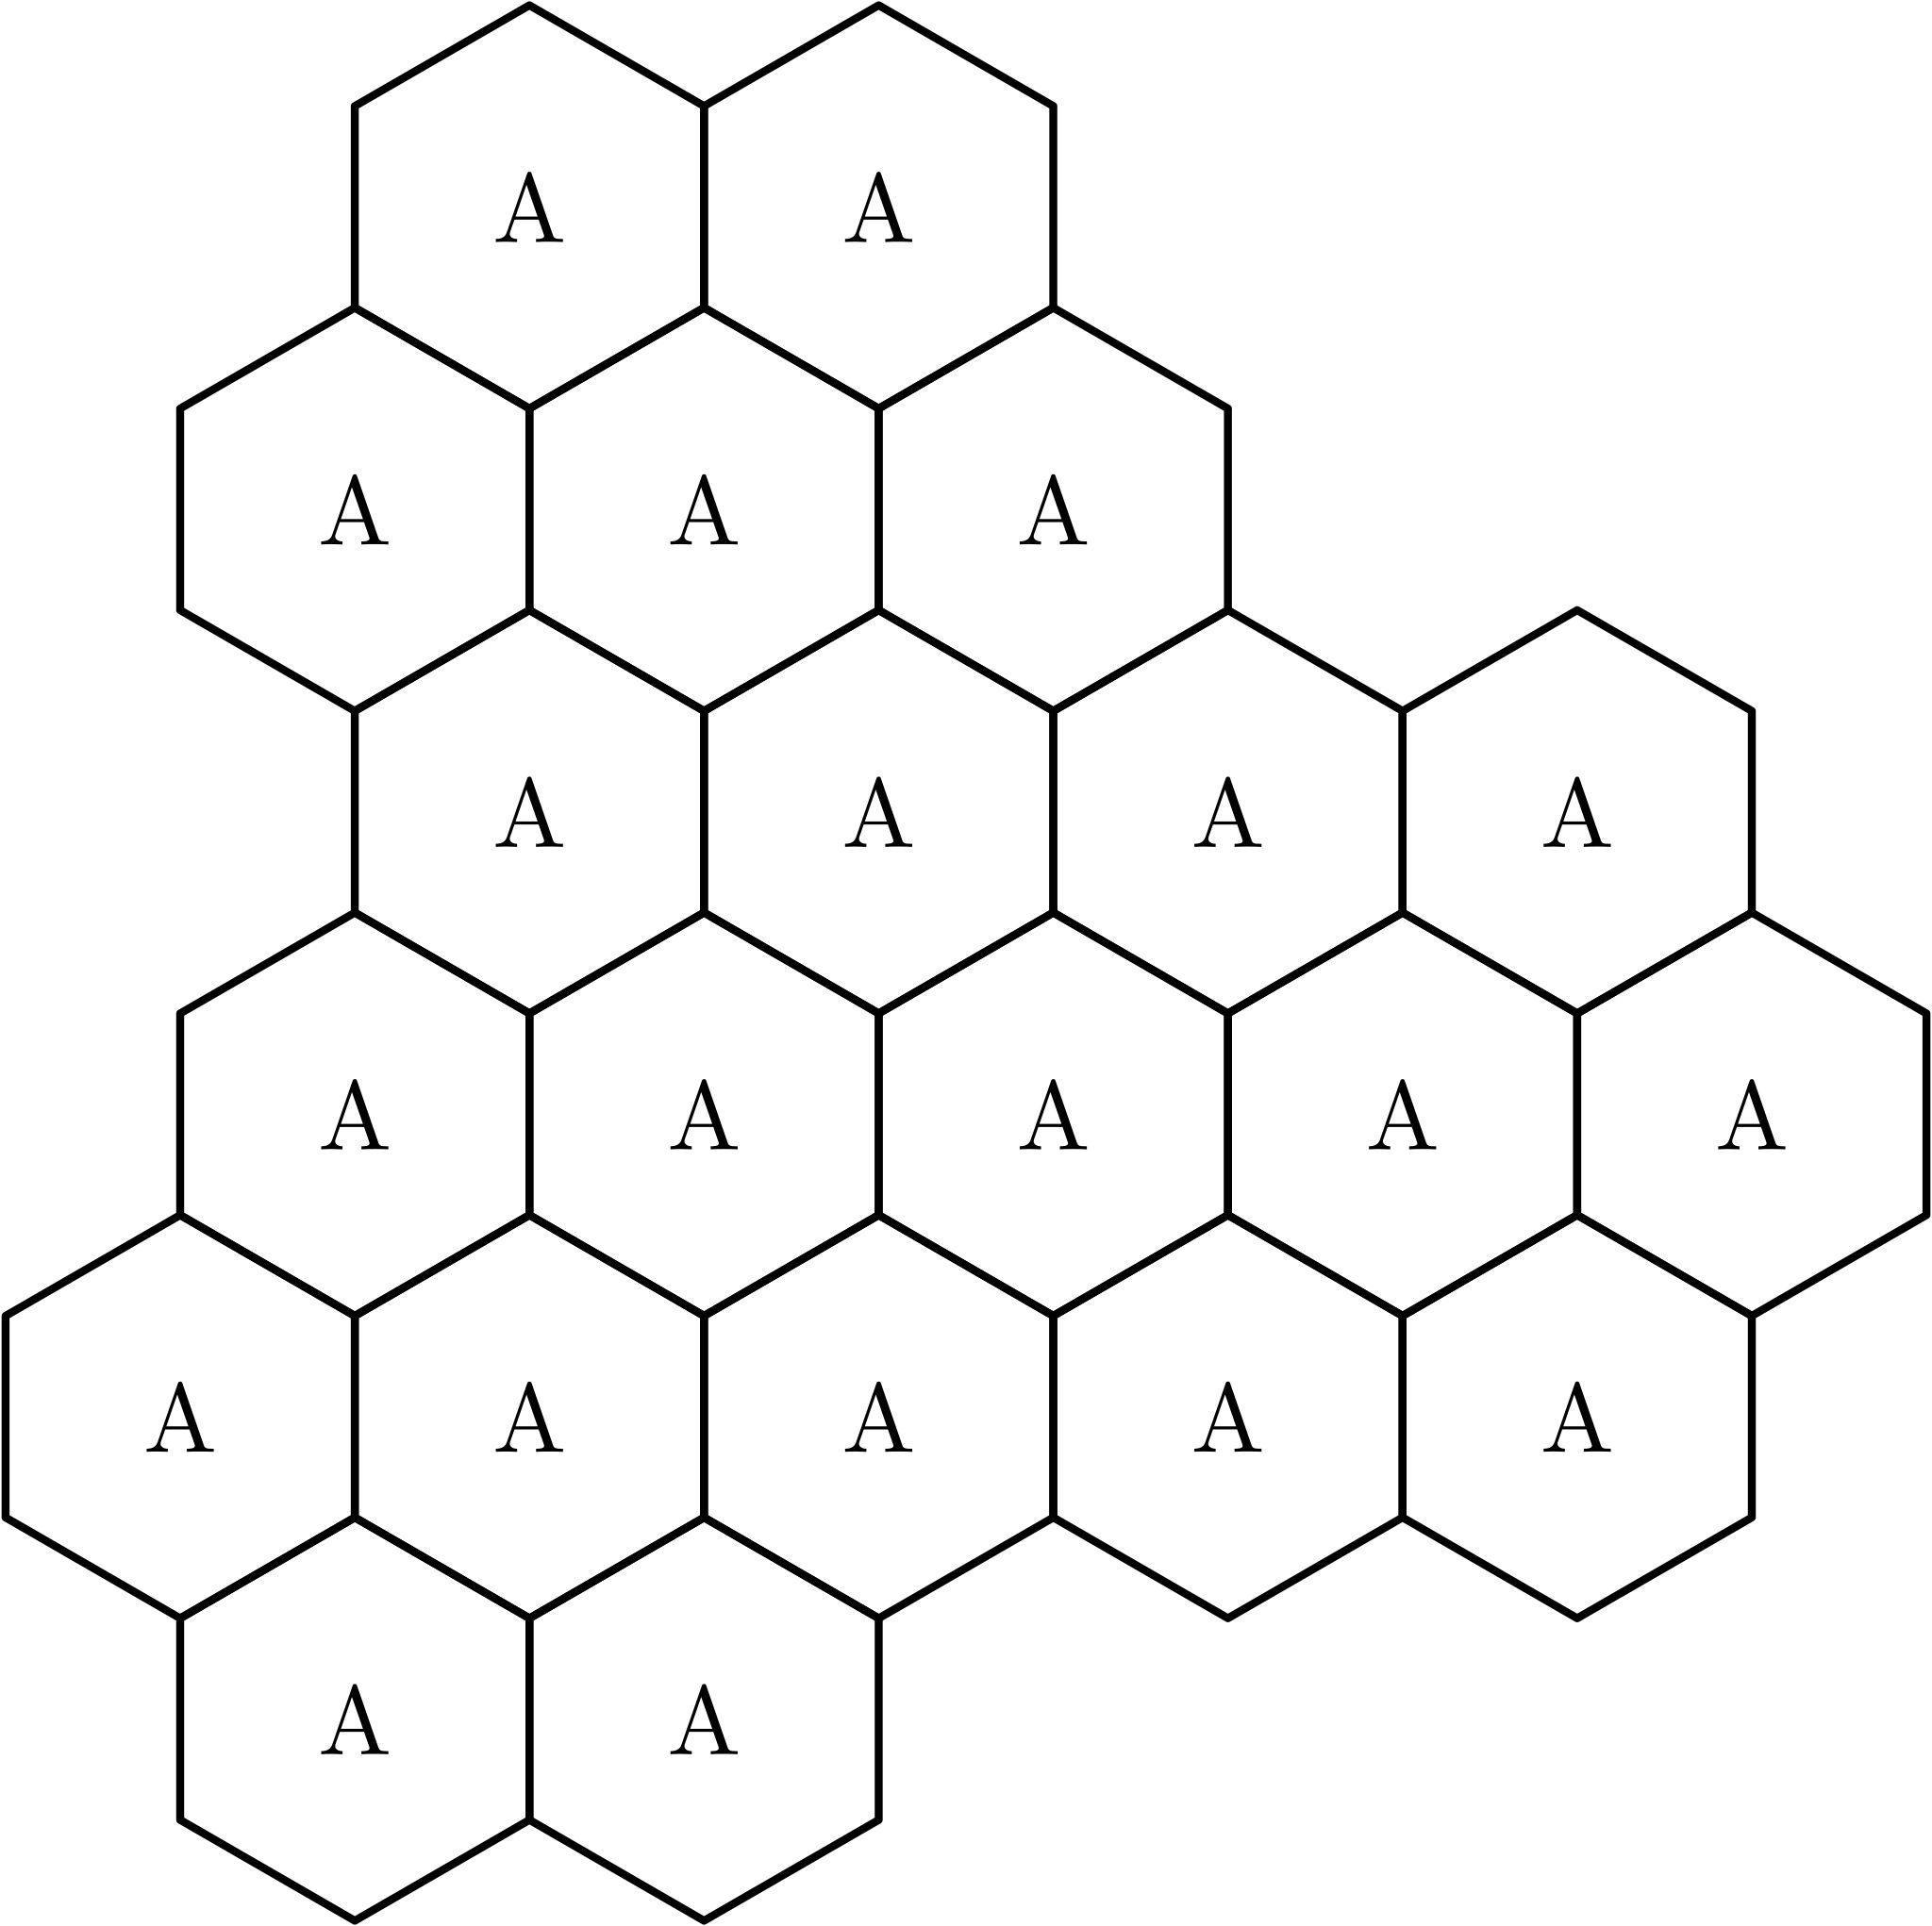
\includegraphics[width=\textwidth]{./ch1/img/universal_freq_reuse.png}
        \caption{Frequency reuse factor of $1$.}
        \label{fig:ufreuse}
    \end{subfigure}
    \caption{Different frequency planning options}
\end{figure}

In the search for higher spectral data rates and a more efficient use of the
resources, \gls{ufr} arises as an alternative in order to make the most out of
the scarce resource that the radio frequency spectrum is. The conventional approach
for cellular networks was to perform a careful frequency planning in order to
avoide the interference among neighboring cells. Clusters of $N$ cells were grouped
together, and assigned $N$ frequency bands to be used, and the pattern is repeated
for different clusters, yielding what is called a \emph{frequency reuse factor}
of $1 / N$, as exemplified in \reff{fig:freuse}.

The problem that this poses is that the available spectrum must be split, which
is an inherent inefficiency in the use of the resources.

\gls{ufr}, in turn, implies that neighboring cells share a common spectrum, as it
can be seen in \reff{fig:ufreuse}, which means that they would be interfering each
other. Therefore, "A new look at the interference" \citep{gesbert10} is needed.

In multi-cell cooperative communications, multiple cells are assumed to cooperate,
in the sense that they take measures in order to alleviate to a certain degree the
level of interference introduced into other parts of the network, or to use that
interference to their advantage. The conventional concept of the interference as
being an impairment shifts to a new point of view where the interference can be
used to improve the overall performance of the network.


% State of the art

% System Model - Block Diagonalization

% Clustering Analysis

% Scheduling

% Conclusions


%%%%%%%%%%%%%%%%%%%%%%%%%%%%%%%%%%%%%%%%%%%%%%%%%%%%%%%%%%%%%%%%%%%%%%%%%%%%%%%%
% REFERENCES
%%%%%%%%%%%%%%%%%%%%%%%%%%%%%%%%%%%%%%%%%%%%%%%%%%%%%%%%%%%%%%%%%%%%%%%%%%%%%%%%
\addcontentsline{toc}{chapter}{\protect\numberline{}{References}}
\bibliographystyle{abbrvnat}
\bibliography{./bibliography/references} 

\end{document}
